\input{/Users/daniel/github/config/preamble.sty}%available at github.com/danimalabares/config

\begin{document}

\begin{minipage}{\textwidth}
	\begin{minipage}{1\textwidth}
		Semin\'ario das Sextas \hfill PUC-Rio
		
		{\small\href{https://github.com/Friday-seminar/}{github.com/Friday-seminar}\hfill\href{https://github.com/danimalabares/seminars}{github.com/danimalabares/seminars}}
		\end{minipage}
\end{minipage}\vspace{.2cm}\hrule

\vspace{10pt}

{\Huge Jacobian elliptic fibrations on K3s \\with a non-symplectic automorphisms of prime order}

\hfill{\Large Felipe Zingali Meira}

\hfill{\Large UFRJ}

\hfill{\large 20 Septembro 2024}

\paragraph{Abstract} K3 surfaces are one of the few classes of algebraic surfaces which allow more than one distinct relatively minimal elliptic fibration. There are distinct ways of classifying such fibrations. In this talk, we will describe how to classify these fibrations with relation to the action of a non-symplectic automorphism $\sigma$ of prime order on a K3 surface $X$, and how each type of fibration relates to a linear system in the quotient surface $X/\sigma$.

\tableofcontents

\begin{figure}[H]
	\centering
	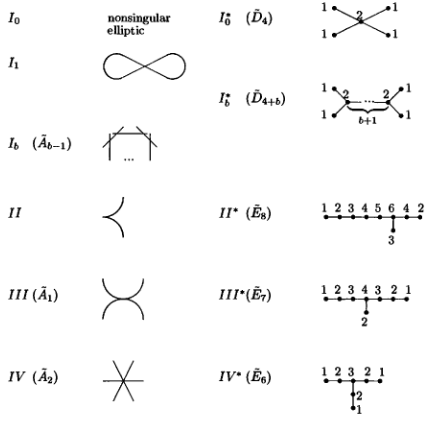
\includegraphics[width=0.6\textwidth]{fig1.png}
	\caption*{\href{https://www.math.columbia.edu/~chaoli/docs/EllipticSurfaces.html}{Kodaira classification of fibers}}
\end{figure}

\section{Definitions}

\begin{defn}
	Let $S$ be a projective smooth surface and $C$ a projective smooth curve. An \textit{\textbf{ elliptic fibration}} is a surfective map $\mathcal{E}:S\to C$ such that
	\begin{enumerate}[label=(\roman*)]
		\item All but finitely many fibres $F_{v}=\mathcal{E}^{-1}$ are irreducible genus 1 curves.
		\item $\mathcal{E}$ is \textit{\textbf{Jacobian}} if there is a section $s_0:C\to  S$.
		\item $\mathcal{E}$ is \textit{\textbf{relatively minimal}} if no fibre contains a $(-1)$-curve.
	\end{enumerate}
\end{defn}

The generic fiber of such a fibration is a genus 1 curve over the function field of the curve $E/K(C)$. Then there is a one-to-one correspondence
\[\{\text{pts in $E(K(x))$}\overset{\text{1-1} }{\longleftrightarrow }\} \{\text{sections $s:C\to S$} \}\]

Drawing of this fibration: base space is a curve, total space is a family of elliptic curves. Section is a curve that takes one point from every elliptic curve in total space.

\begin{enumerate}
	\item $K_S=(\chi(s)-2)F$,  $F$ is the fiber class in $\operatorname{NS}(S)$. Recall that Neron-Severi group is divisors quotient linear equivalence, but in this case perhaps we can just take it to be Picard group.
\item $\operatorname{NS}(S)$ is a lattice with the intersection pairing.
	\item $\operatorname{Triv}(S)=\left<\Sigma_0,F\right> \oplus \left<\text{components of reducible fibers} \right> $.
		\[\dfrac{\operatorname{NS}(S)}{\operatorname{Triv}(S)}\cong E(K(C))\]
		and also we have the formula
		\[\rho(S)=2+r+\sum m_v-1\]
	\item $e(S)=\chi_{\text{tod} }(S)=\sum_{v\in C}e^{F_v}$ where $\chi(S)=\frac{e(S)}{12}+k^2_S$
	\item 
\end{enumerate}

\section{Rational elliptic surfaces}

\begin{defn}
	Let $R$ be a rational surface (nonsingular projective) with an elliptic fibration $\mathcal{E}:R\to \mathbb{P}^1$.
\end{defn}

\begin{example}
	Let $f,g$ be cubics in  $\mathbb{P}^2$ and take the rational map
	\begin{align*}
		\varphi: \mathbb{P}^2 &\overset{\operatorname{rat}}{\longrightarrow} \mathbb{P}^1 \\
		p &\longmapsto [f(p):g(p)]
	\end{align*}
	\[\begin{tikzcd}
	&R\arrow[dl,"\eta",swap]\arrow[dr,"\mathcal{E}"]\\
	\mathbb{P}^2\arrow[rr,"\varphi"]&&\mathbb{P}^1
	\end{tikzcd}\]
\end{example}

\paragraph{Over $k=\bar{k}$} Every RES which is rel. min. + Jacobian is constructed by blowing up the base points of a cubir pencil. $\rho(R)=10$.

\section{K3 surfaces}

\begin{quotation}
	An important subclass of K3 surfaces, easier to analyze than the general case, consists of the K3 surfaces with an elliptic fibration $X\to \mathbb{P}^1$. "Elliptic" means that all but finitely many fibers of this morphism are smooth curves of genus 1. The singular fibers are unions of rational curves, with the possible types of singular fibers classified by Kodaira.
	
	\hfill \href{https://en.wikipedia.org/wiki/K3_surface#Elliptic_K3_surfaces}{wiki}
\end{quotation}


\begin{defn}
	A \textit{\textbf{K3 surface}} is a smooth projective surface such that
	\begin{itemize}
	\item $q(X):=h^1(X,\mathcal{O}_X)=0$.

	\item $K_X=0$, ie. there exists  $\omega_X\in H^{0}(X,\Omega^2_X)$ non-vanishing.
	\end{itemize}
\end{defn}

\begin{prop}
	$\mathcal{E}:X\to \mathbb{P}^1$ Jacobin, rel. min. Then
	\[X \text{ is a K3}\iff e(X)=24 \]
	\[q(X)= h^{1}(X,\mathcal{O}_X)=h^{2}(X,\mathcal{O}_X)+h^{0}(X,\mathcal{O}_X)-\chi(X)=1+1-2=0\]
\end{prop}

\begin{defn}
Let $X$ be a K3 surface and $\sigma\in\operatorname{Aut}(X)$ such that
\[\sigma ^*(\omega_X)=\xi \omega_X,\qquad \xi \text{ root of unity,} \]
We say 
\begin{itemize}
\item $\sigma$ is \textit{\textbf{symplectic}} if $\xi =1$.
\item $\sigma$ is \textit{\textbf{non-symplectic}} otherwise.
\end{itemize}

Suppose $\sigma\in\operatorname{Aut}(X)$ with finite order $\operatorname{ord}\sigma=n$.
\[X/\sigma=\begin{cases}
	\text{K3 if $\sigma$ is symplectic}\\
	\text{Rational if $n\geq 3$ or $n=2$ and $\operatorname{Fix}(\sigma)\neq \varnothing $}\\
	\text{Enrigues if $n=2$ and $\operatorname{Fix}(\sigma)=\varnothing $} 
	\qquad &
\end{cases}\]
\end{defn}

\section{Base change}

How to build K3 surfaces out of…

\[\mathcal{E}:R\to \mathbb{P}^1,\qquad \qquad \tau :\mathbb{P}^1\to \mathbb{P}^1 \text{ $n-1$ cover} \]
\[\begin{tikzcd}
	R\arrow[d,"\mathcal{E}",swap]& R\times_{\mathbb{P}^1}\mathbb{P}^1\arrow[l]\arrow[d]& Y\arrow[d]\\
	\mathbb{P}^1&\mathbb{P}^1\arrow[l,"\tau ",swap]& X\arrow[l,swap,"\mathcal{E}_X"]
\end{tikzcd}\]

\begin{remark}[Sergey]\leavevmode
	That fibered product may have singularities at the critical points of $\mathcal{E}$ and $\tau$, ie. any point that is collapsed in the quotient (definition of fibered product).
\end{remark}

	We can tell the Kodaira type of a fiber $\mathcal{E}^{-1}_X(v)=F^X_v$ by knowing
	\begin{itemize}
	\item the kodaira type of $\mathcal{E}^{-1}(u):=F_u$, $u=\tau(v)$.
	\item The ramification index $r(v|u)$
	\end{itemize}

	There are tables on how to determine the Kodaira types from that.

*Several drawings*

\paragraph{$n=3$} $\mathcal{E}_{x}:X\to \mathbb{P}^1$ is a K3 if
\begin{itemize}
\item $F_a^x$ is of type IV or $I^*_n$ and $F^x_b$ is at type $I_n, \operatorname{I I},\operatorname{I I I }$.
\end{itemize}

\section{Towards the classification}

\begin{defn}
$(X,\sigma)$, $X$ a K3 surface, $\sigma\in\operatorname{Aut}(X)$, $\operatorname{ord}(\sigma)=p$ prime, $\sigma$ non-symplectic. $\mathcal{E}:X\to \mathbb{P}^1$ a Jacobian ell. fib. (by K3 surface condition it is relatively minimal via adjunction formula). Then

\begin{itemize}
\item $\mathcal{E}$ is of \textit{\textbf{type 1}} if $\sigma^*(F)=F$ and $\sigma$ acts trivially on $\mathbb{P}^1$.
\item $\mathcal{E}$ of \textit{\textbf{type 2}} if  $\sigma^*(F)=F$ and $\sigma$ acts on $\mathbb{P}^1$ with order $p$.
\item $\mathcal{E}$ is of \textit{\textbf{type 3}} if $\sigma^*(F)\neq F$.
\end{itemize}
\end{defn}

Three drawings to show the types. Type one moves a point in a fiber to a another point the fiber, while fixing the base point of the fiber. Type 2 moves points from one fiber to another, and also maps the base points one to another. Type 3 is more messy, moves points from a fiber to the horizontal curves (sections)

\paragraph{Assumption:} acts trivially on $\operatorname{NS}(X)$ (Sarti, Arteloni, Taki).

\subsection{Type 1}
$F_v$ nonsingular, $\sigma$ acts on $F_v$ the order of an automorphism of an elliptic curve is 2,3,4,6 the order of an automorphism of an elliptic curve is 2,3,4,6.

When $p=2$, Garbognati, Salgado 17, Fibre types of  $F_v$ are $\operatorname{I}n,\operatorname{I}n^* ,\operatorname{I I I}$.

When $p=3$, 24, and types $\operatorname{I},\operatorname{I I}^* ,\operatorname{IV},\operatorname{IV}^* ,\operatorname{I}_{0},\operatorname{I}_{0}^*$.

$X/\sigma$, $\operatorname{ord}(\sigma)\geq 3$. Then $\operatorname{Fix}(\sigma)$ allows isolated fixed points
\[\operatorname{Fix}(\sigma)=C^1_g \cup c_1\cup \ldots \cup c_n\cup \{p_1,\ldots,p_k\}\]
where $C^1_g$ is a curve of genus $g$ and $C_1,\ldots,C_k$ are rational curves.

When $p=2$, $\operatorname{Fix}(\sigma)\neq \varnothing$.

$X/\sigma=\tilde{R}$ is rational and smooth.
\[\begin{tikzcd}
	\tilde{R}\arrow[d]&\tilde{X}\arrow[l,"\hat{\pi}"]\arrow[d]\\
	X/\sigma & X\arrow[l,"\pi"]
\end{tikzcd}\]

$ \mathcal{E}:X\to \mathbb{P}^1$ induces a linear system of curves $\Lambda$ in $\tilde{R}$.

\begin{enumerate}
	\item  $\mathcal{E}$ of type 1 $\implies \Lambda$ pencil of conics.
	\item $\mathcal{E}$ of type 2 $\implies \Lambda$ pencil of genus 1 curves.
	\item $\mathcal{E}$ of type 3 $\implies \Lambda$ is a non-complete linear system.

	\item 
\end{enumerate}

\subsection{Type II}

*Computations and discussion*

$\mathcal{E}:X\to \mathbb{P}^1$ of type  II induces a Jacobian elliptic fibration. $\mathcal{E}_{\tilde{R}}:\tilde{R}\to \mathbb{P}^1$ blow down to a rel. minimal $\mathcal{E}_R:R\to \mathbb{P}^1$.

Let $\tau :\mathbb{P}^1\to \mathbb{P}^1$ be the quotient by the action of $\sigma$ in $\mathbb{P}^1$.
\[\begin{tikzcd}
	R\arrow[d,swap,"\mathcal{E}_R"]& R\times_{\mathbb{P}^1}\mathbb{P}^1\arrow[l]\arrow[d]\\
	\mathbb{P}^1&\mathbb{P}^1\arrow[l,"\tau "]
\end{tikzcd}\]
I obtain $\mathcal{E}:X\to \mathbb{P}^1$ back.

Let $F_a^X,F_b^X$ be the ramified fibers of $\mathcal{E}:X\to \mathbb{P}^1$ of type 2. $\operatorname{ord}(\sigma)=3$.
\begin{itemize}
\item $F^X_a$ is of type $\operatorname{I}^*_{3n}$ or $\operatorname{I}_{0}$.
\item $F^X_b$ is of type $\operatorname{I}_{3n},\operatorname{I}^*_{0}$ or $\operatorname{I I I}$.
\item Every other fibre is irreducible.

	*Drawing using a base change*
\end{itemize}

\section{A concrete example of everything happening}

Start by building a rational elliptic surface, base change it, look at the K3 surface that's going to appear, and this K3 look at different elliptic fibrations and see what types they will have.

Start with $\mathbb{P}^2$ and
\begin{align*}
	f:xyz&=0\\
	g:(x-y)(y-z)(z-x)&=0
\end{align*}

Drawings of these curves and then of the K3 surface obtained after base change. The reasons why the intersections are as drawn is more involved.

$\Gamma$ pencil of curves in $\mathbb{P}^2$ induced by $\mathcal{C}_{|M'|}:X\to \mathbb{P}^1$ 
\begin{itemize}
\item $\mathcal{C}_{a}$ image of $\mathcal{G}_{a}$.

\item $\mathcal{C}_{0}$ image of $\mathcal{G}_{a}$ 

	These two imply $\Gamma:s\mathcal{C}_{a}+t\mathcal{C}_{b}$ 

\item The generic fibre of $\mathcal{C}_{|M'|}$ is given by
	\[s^3\mathcal{C}_a+t^3\mathcal{C}_b\]
	\[y^2=x^3+A(t^3)x+B(t^3)\]
	\[(x,y,t)\mapsto (x,y,\xi_3t\]
\end{itemize}

*I had to leave the talk*
\end{document}
